\documentclass{article}
\usepackage{graphicx}
\usepackage{amsmath}
\usepackage{subfigure}

\begin{document}

\begin{figure}[ht]
\centering

%
\subfigure
[
A trace.
]
{
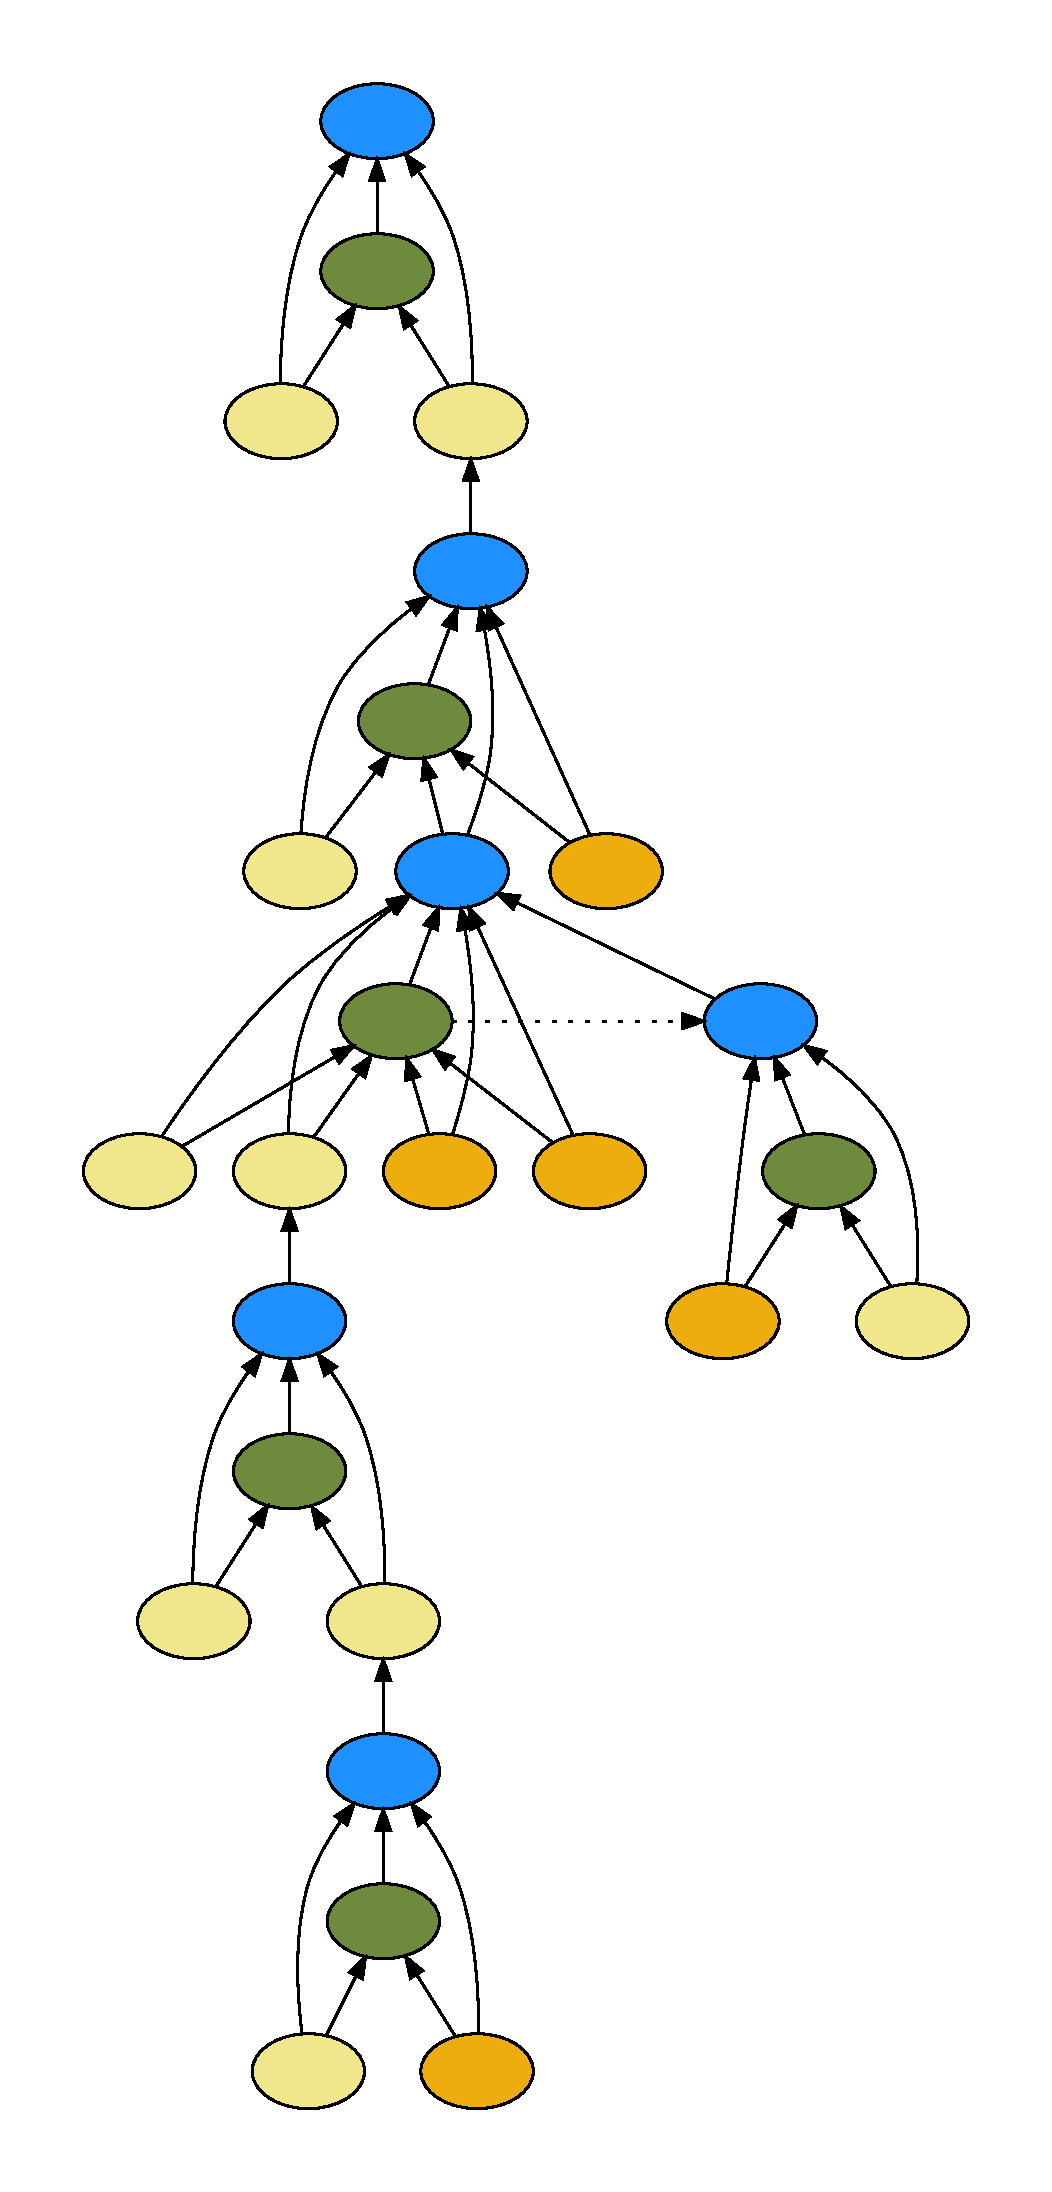
\includegraphics[width=200pt,height=200pt]{partition/dot0.pdf}

\label{fig:partition_rho}
}

\quad

\subfigure
[
The scaffold partitions the trace into five groups: the nodes that will definitely still exist in the proposal trace but whose values may change (drg), the nodes that we will definitely compute likelihoods at (absorbing), the nodes that may no longer exist (the brush), the parents of nodes in these three groups (parents), and all other nodes which need never be visited at all (ignored). Note that future graphs will not distinguish between these last two groups.
]
{
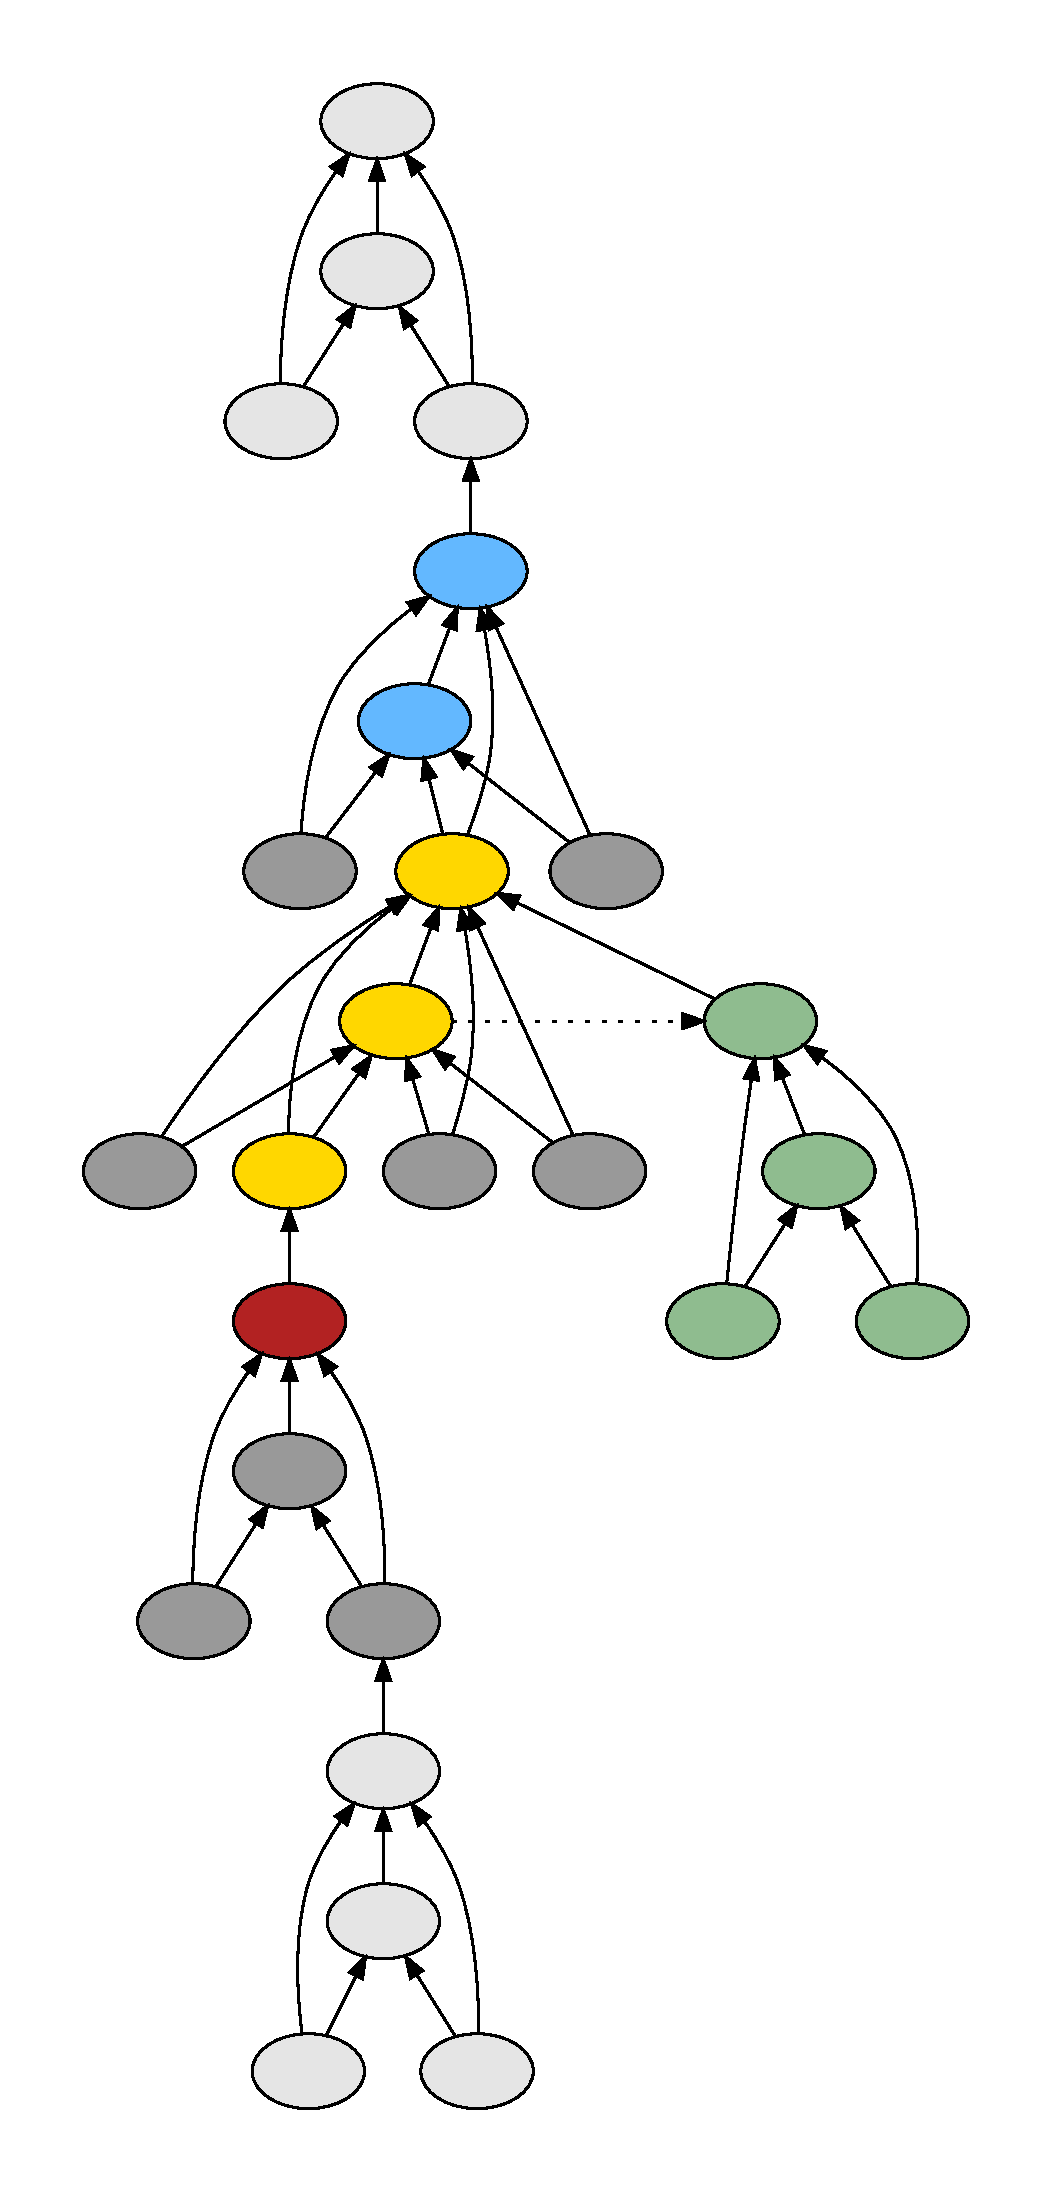
\includegraphics[width=200pt,height=200pt]{partition/dot20.pdf}
\label{fig:partition_scaffold}

}

%

\caption{Partitioning the trace along a scaffold}

\label{fig:partition}
\end{figure}



%%%%%%%%%%%%%%%%%%%%%%%%%%%%%%%%
%%%%%%%%%%%%%%%%%%%%%%%%%%%%%%%%
%%%%%%%%%%%%%%%%%%%%%%%%%%%%%%%%
\begin{figure}[ht]
\centering

%
\subfigure
[
To construct a scaffold, we first walk downstream from the principal node, and color gold every node
whose value may change, and blue every node at which we can
absorb.
]
{
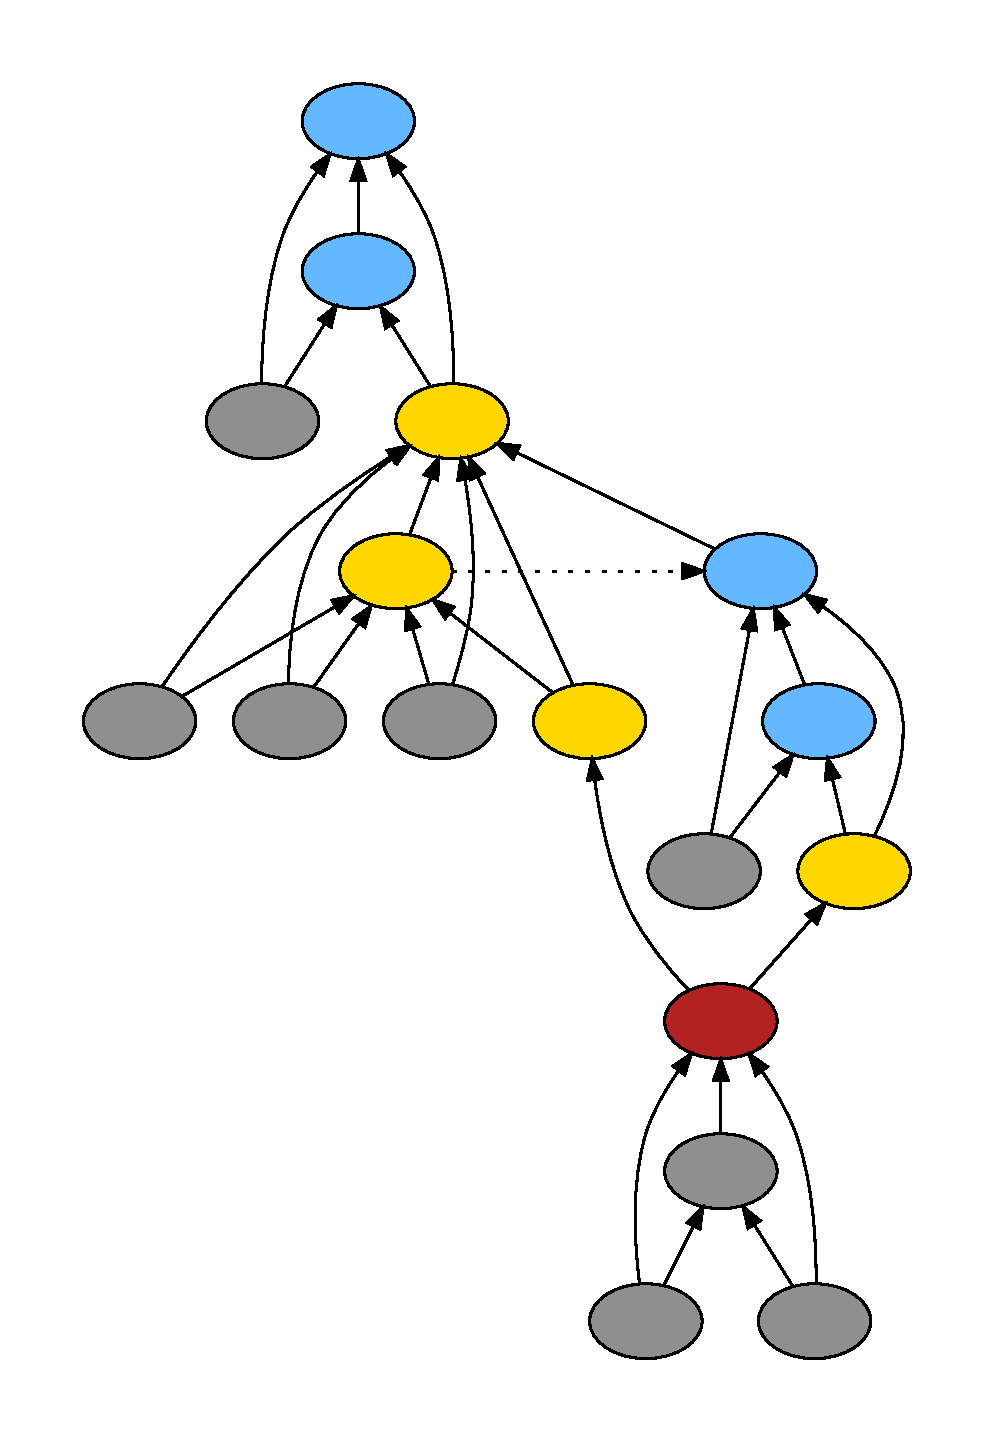
\includegraphics[width=200pt,height=200pt]{erg_to_drg/dot4.pdf}

\label{fig:scaffold_extended}
}

\quad

\subfigure
[
Next, we color green every node that may no longer exist once
the gold nodes are resampled. At this point, the red and gold nodes 
constitute the definite regeneration graph, the blue nodes constitute the absorbing border, and the green nodes constitute the brush.
]
{
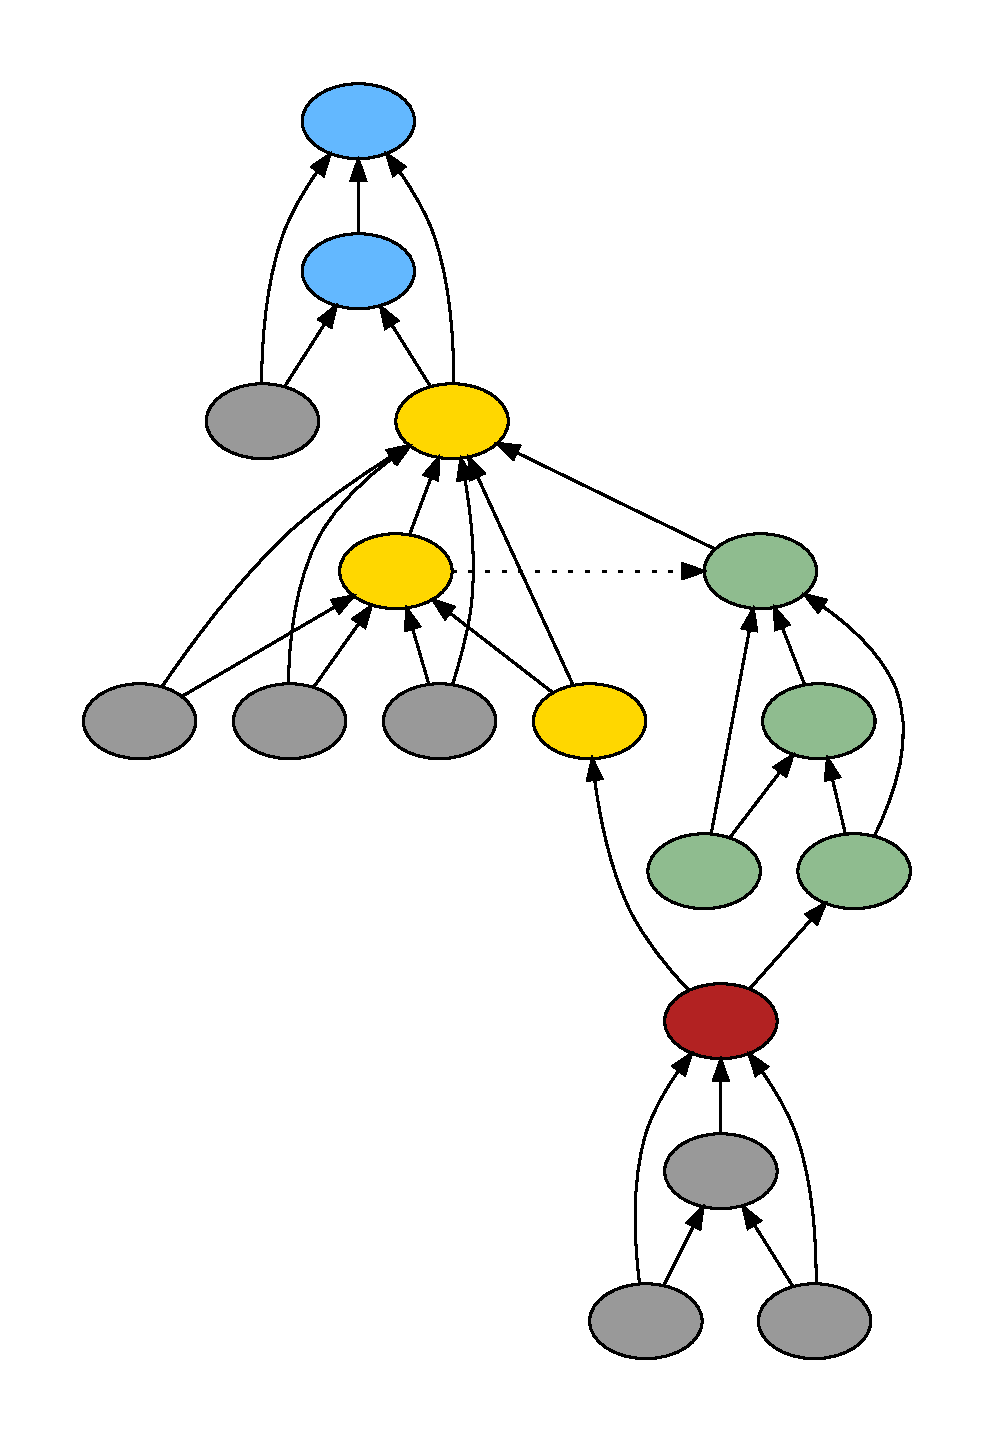
\includegraphics[width=200pt,height=200pt]{erg_to_drg/dot2.pdf}
\label{fig:scaffold_disabled}

}

%

\caption{The two stages of constructing a scaffold}

\label{fig:scaffold}
\end{figure}


%%%%%%%%%%%%%%%%%%%%%%%%%%%%%%%%%%
%%%%%%%%%%%%%%%%%%%%%%%%%%%%%%%%%%
%%%%%%%%%%%%%%%%%%%%%%%%%%%%%%%%%%

\begin{figure}[ht]
\centering

\subfigure
[
A torus with two border nodes. Suppose we regenerate the higher one first, and one of the nodes regenerated makes a simulation request. 
Regen then hands over control to eval in order to evaluate the expression. 
(TODO mark the three nodes that have values, and space-permitting have an
 extra figure to start that just shows the scaffold.)
]
{
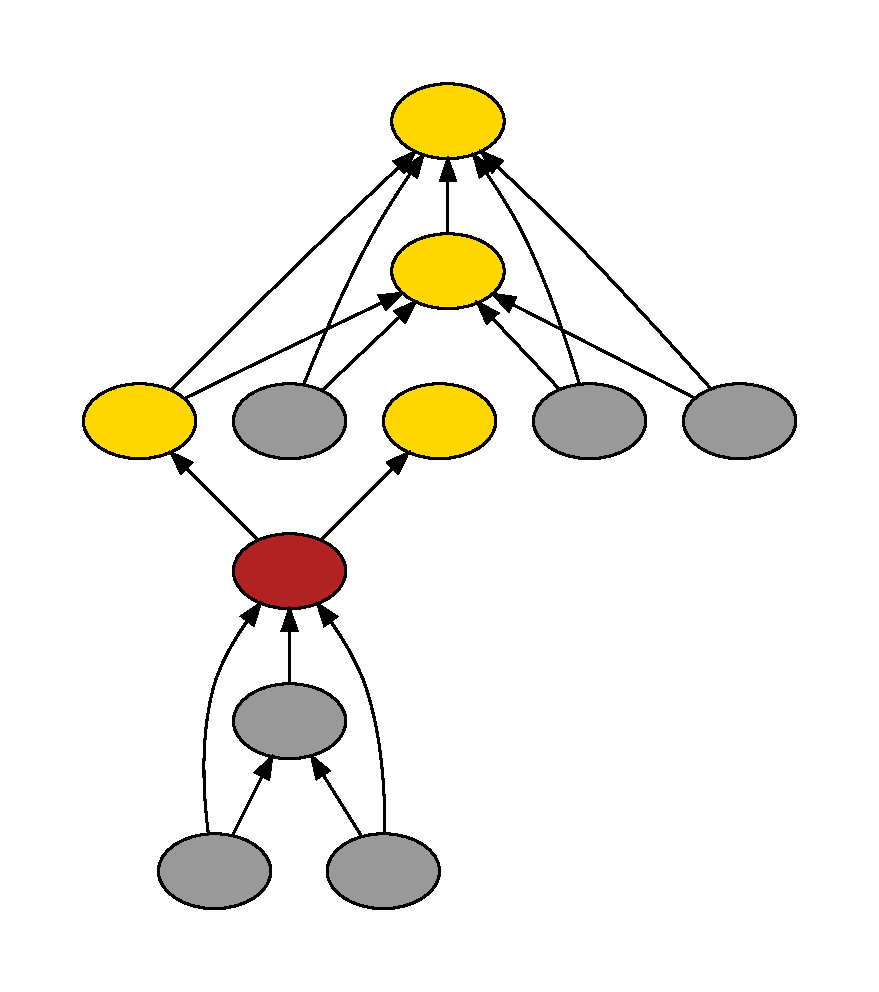
\includegraphics[width=200pt,height=200pt]{regen_to_eval_to_regen/dot6.pdf}

\label{fig:rer_torus}
}

\quad

\subfigure
[
 Evaluating the expression might involve referencing other nodes in the trace, for example to resolve a variable lookup. Those nodes may be in the drg and may not have been regenerated yet, so eval must hand over control to regen to guarantee that all values have been regenerated before they are used.
]
{
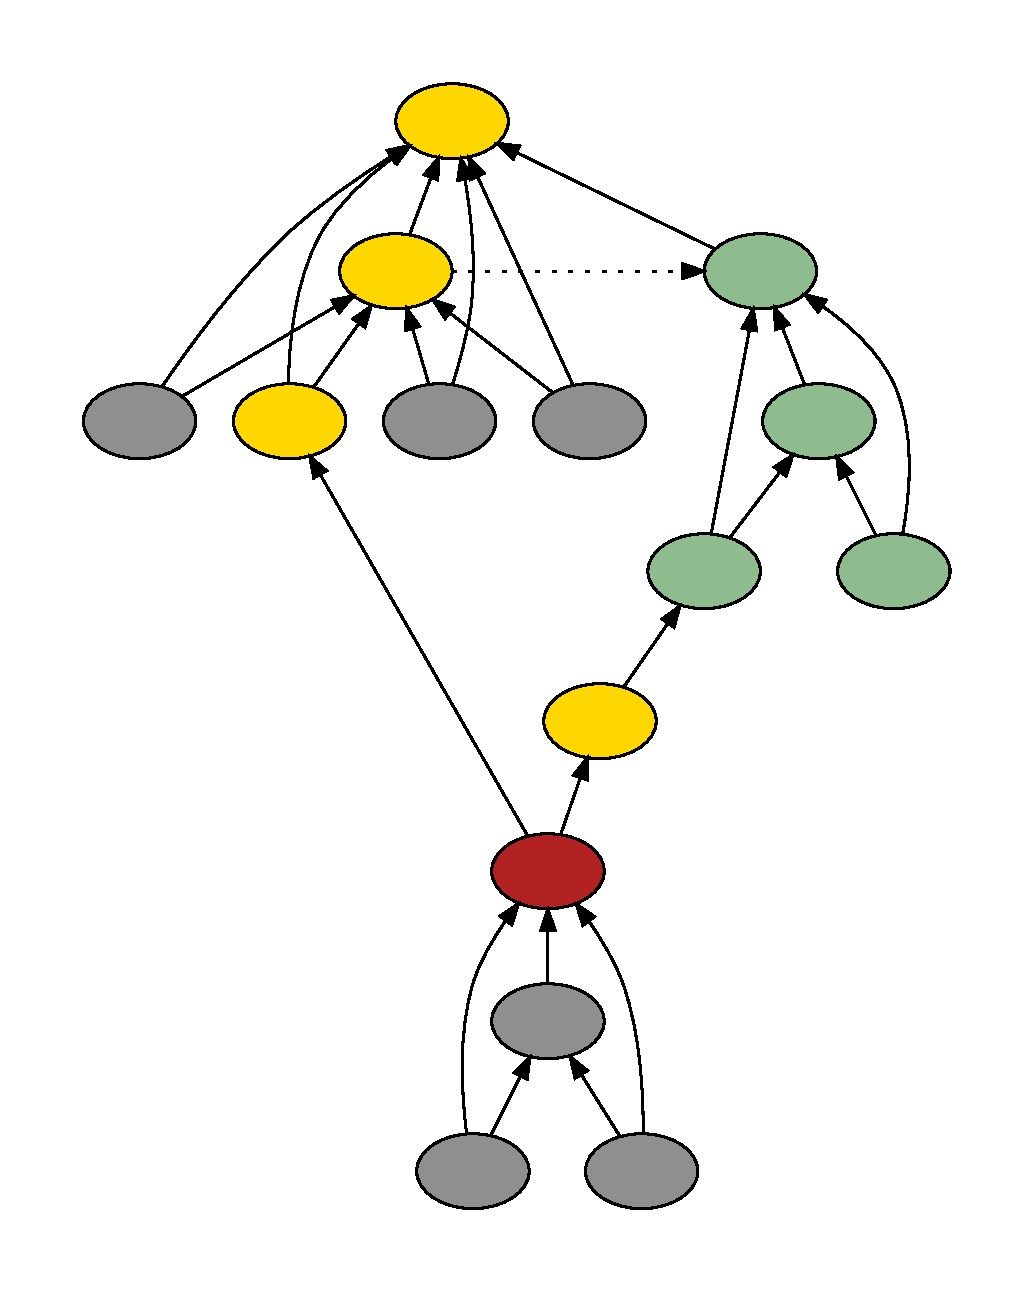
\includegraphics[width=200pt,height=200pt]{regen_to_eval_to_regen/dot2.pdf}
\label{fig:rer_full}

}

%

\caption{Interlacing calls to regen with calls to eval}

\label{fig:rer}
\end{figure}

%%%%%%%%%%%%%%%%%%%%%%%%%%%%%%%%%%
%%%%%%%%%%%%%%%%%%%%%%%%%%%%%%%%%%
%%%%%%%%%%%%%%%%%%%%%%%%%%%%%%%%%%

\begin{figure}[ht]
\centering

\subfigure
[
A large scaffold for sampling a hyperparameter.
]
{
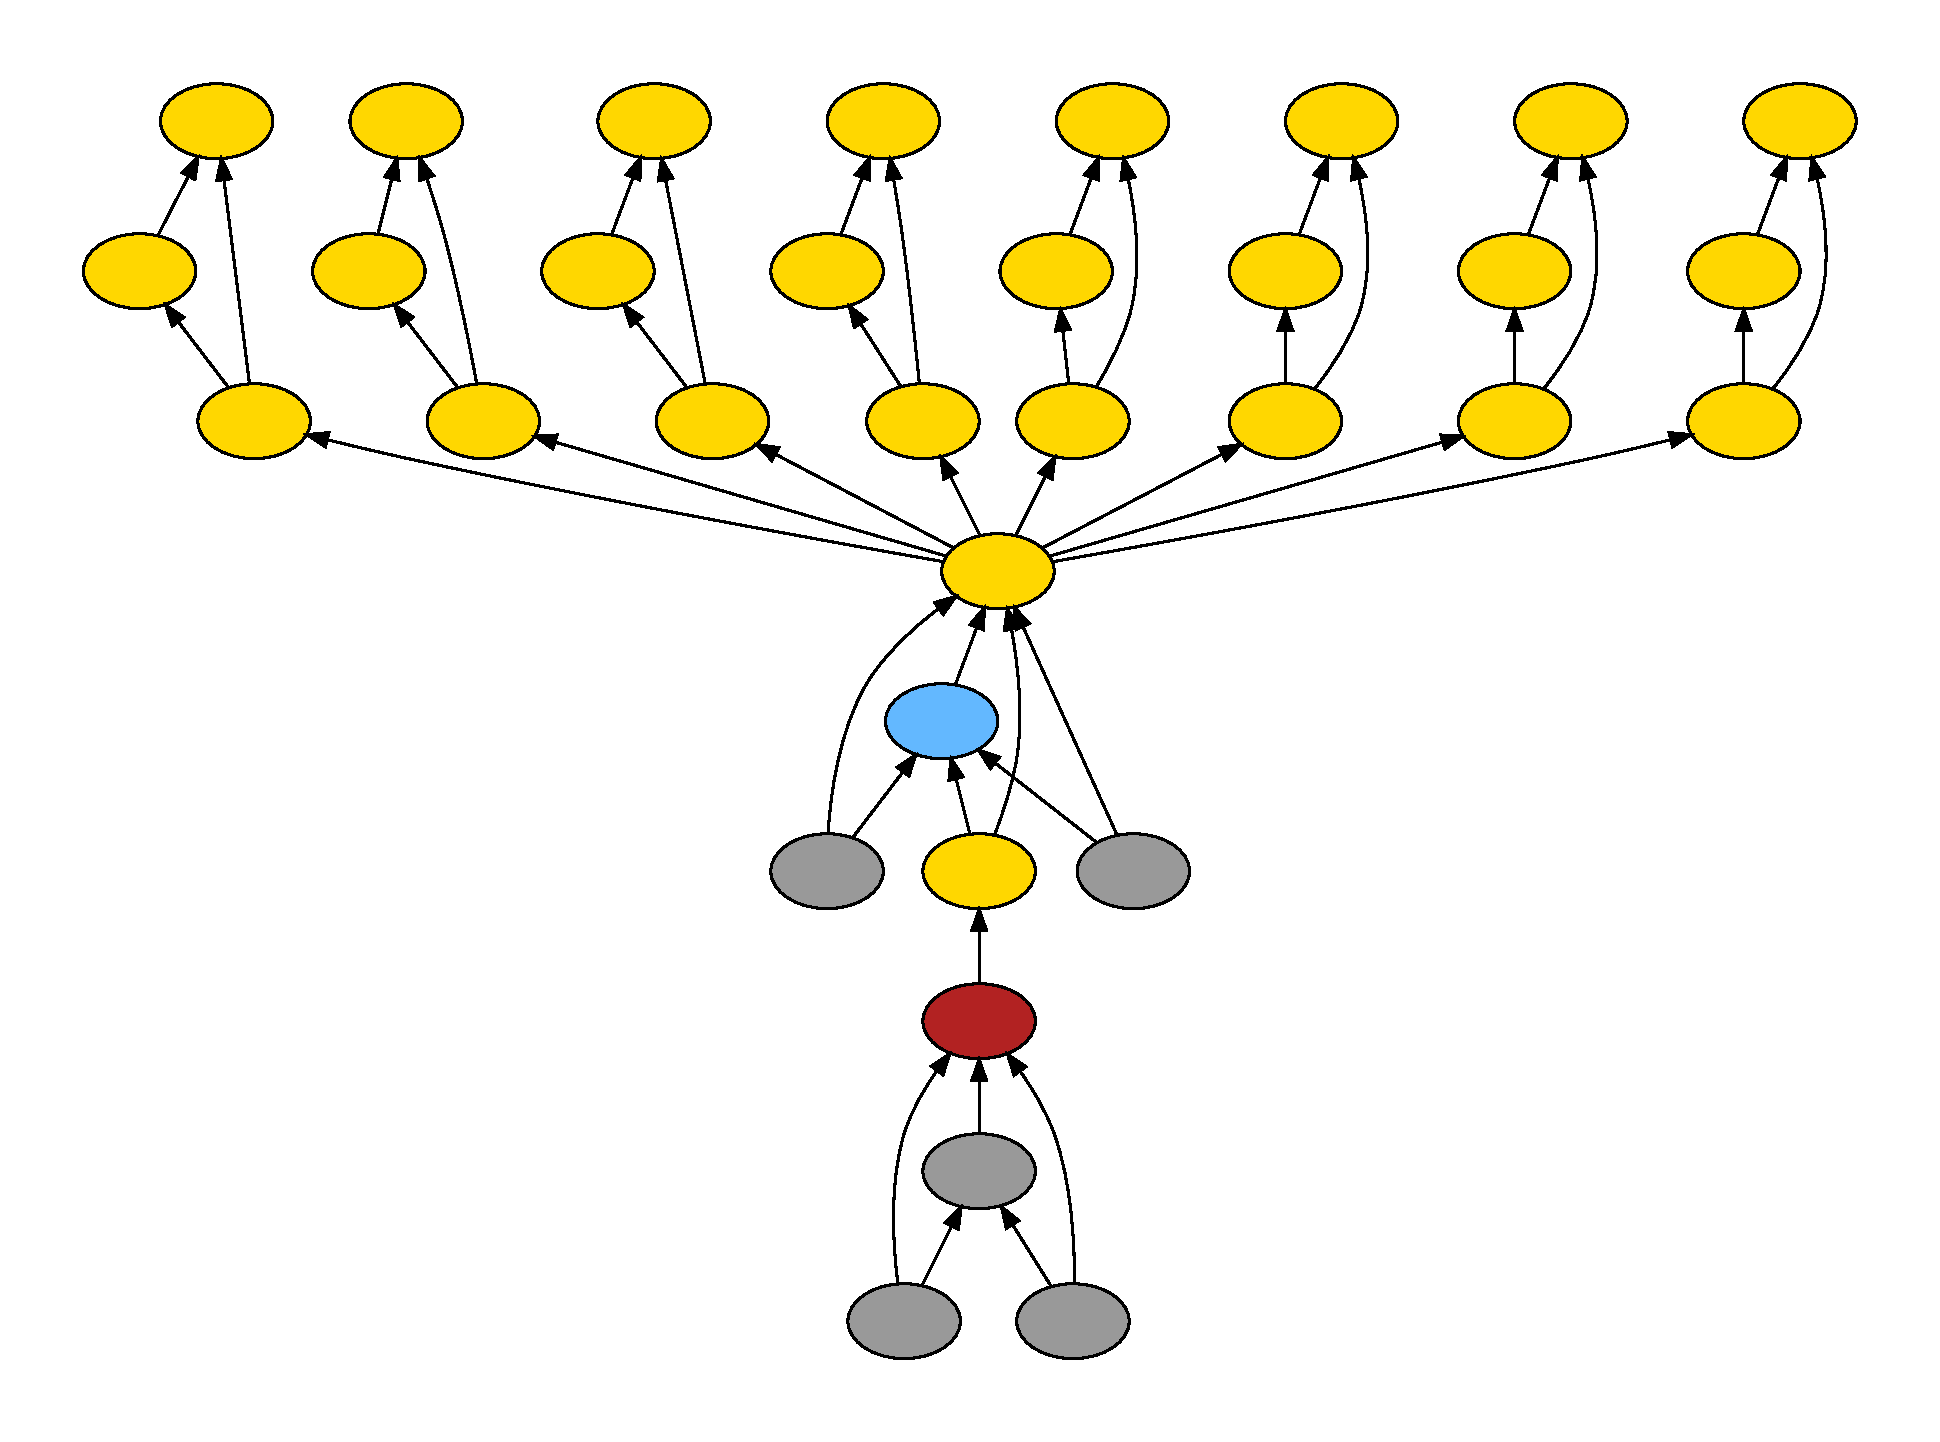
\includegraphics[width=200pt,height=200pt]{aaa_basic_no_aaa/dot2.pdf}
\label{fig:aaa_basic_no_aaa}

}

\quad

\subfigure
[
The application of the maker SP computes the log density of all of its applications for us. We say that the maker SP ``absorbs at applications''.
]
{
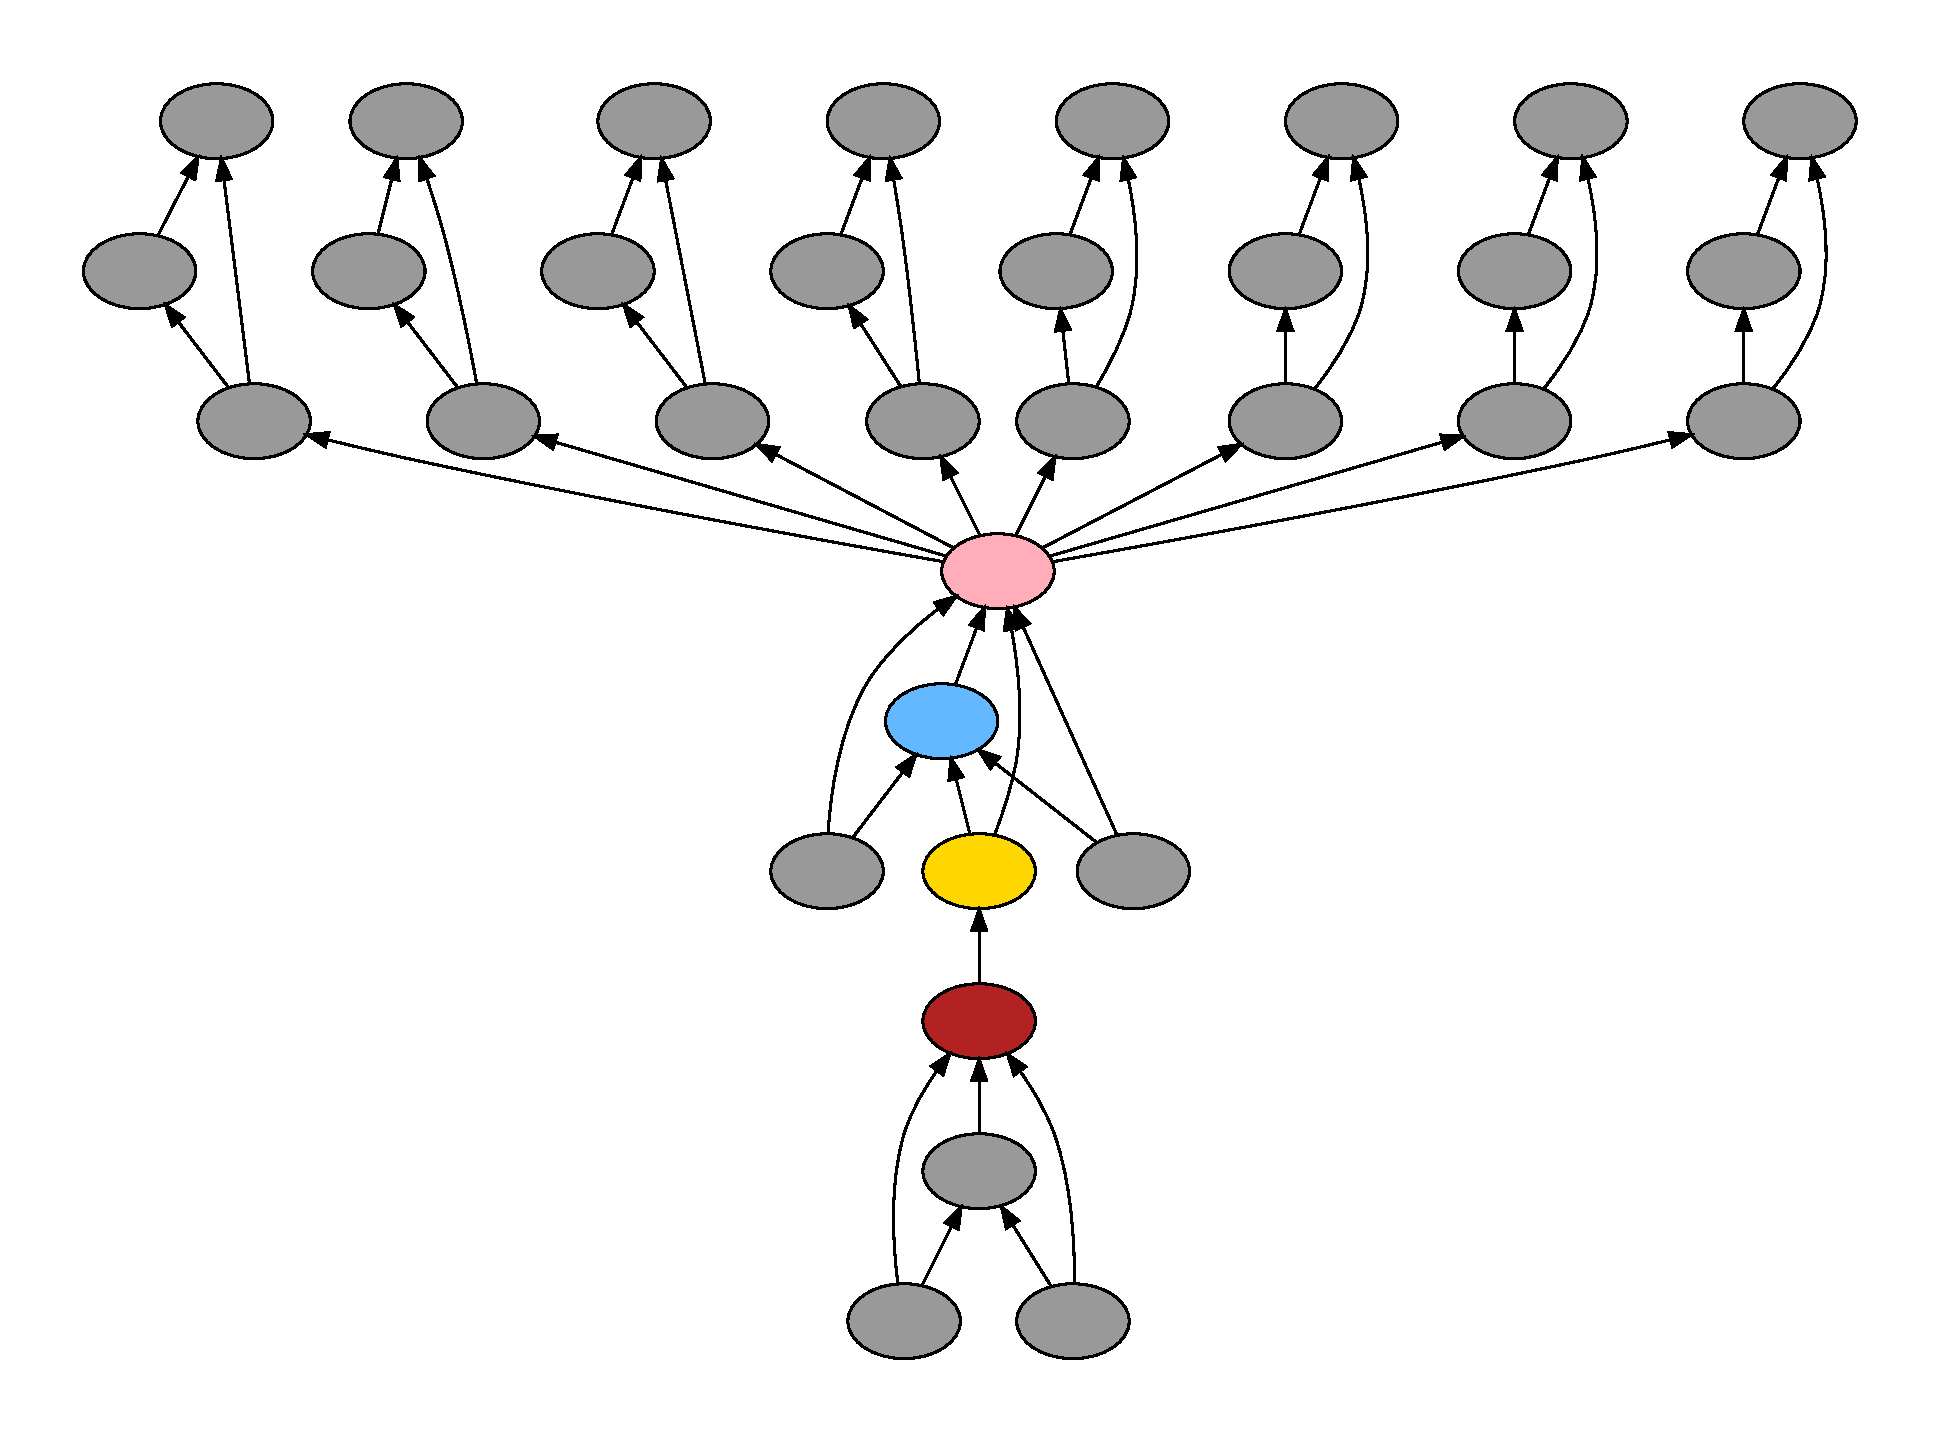
\includegraphics[width=200pt,height=200pt]{aaa_basic_with_aaa/dot2.pdf}
\label{fig:aaa_basic_with_aaa}

}
%

\caption{Absorbing at applications (AAA)}

\label{fig:aaa_basic}
\end{figure}

%%%%%%%%%%%%%%%%%%%%%%%%%%%%%%%%%%
%%%%%%%%%%%%%%%%%%%%%%%%%%%%%%%%%%
%%%%%%%%%%%%%%%%%%%%%%%%%%%%%%%%%%


\begin{figure}[ht]
\centering

\subfigure
[
A scaffold with three border nodes, one of which is absorbing at applications. The child of the aaa node is a reference to it, and would normally be in the drg. (TODO the extended drg and the extended scaffold should refer to the semantic drg/scaffold, before the aaa shortcut, even though it is never constructed. We should abandon the old use of that term)
]
{
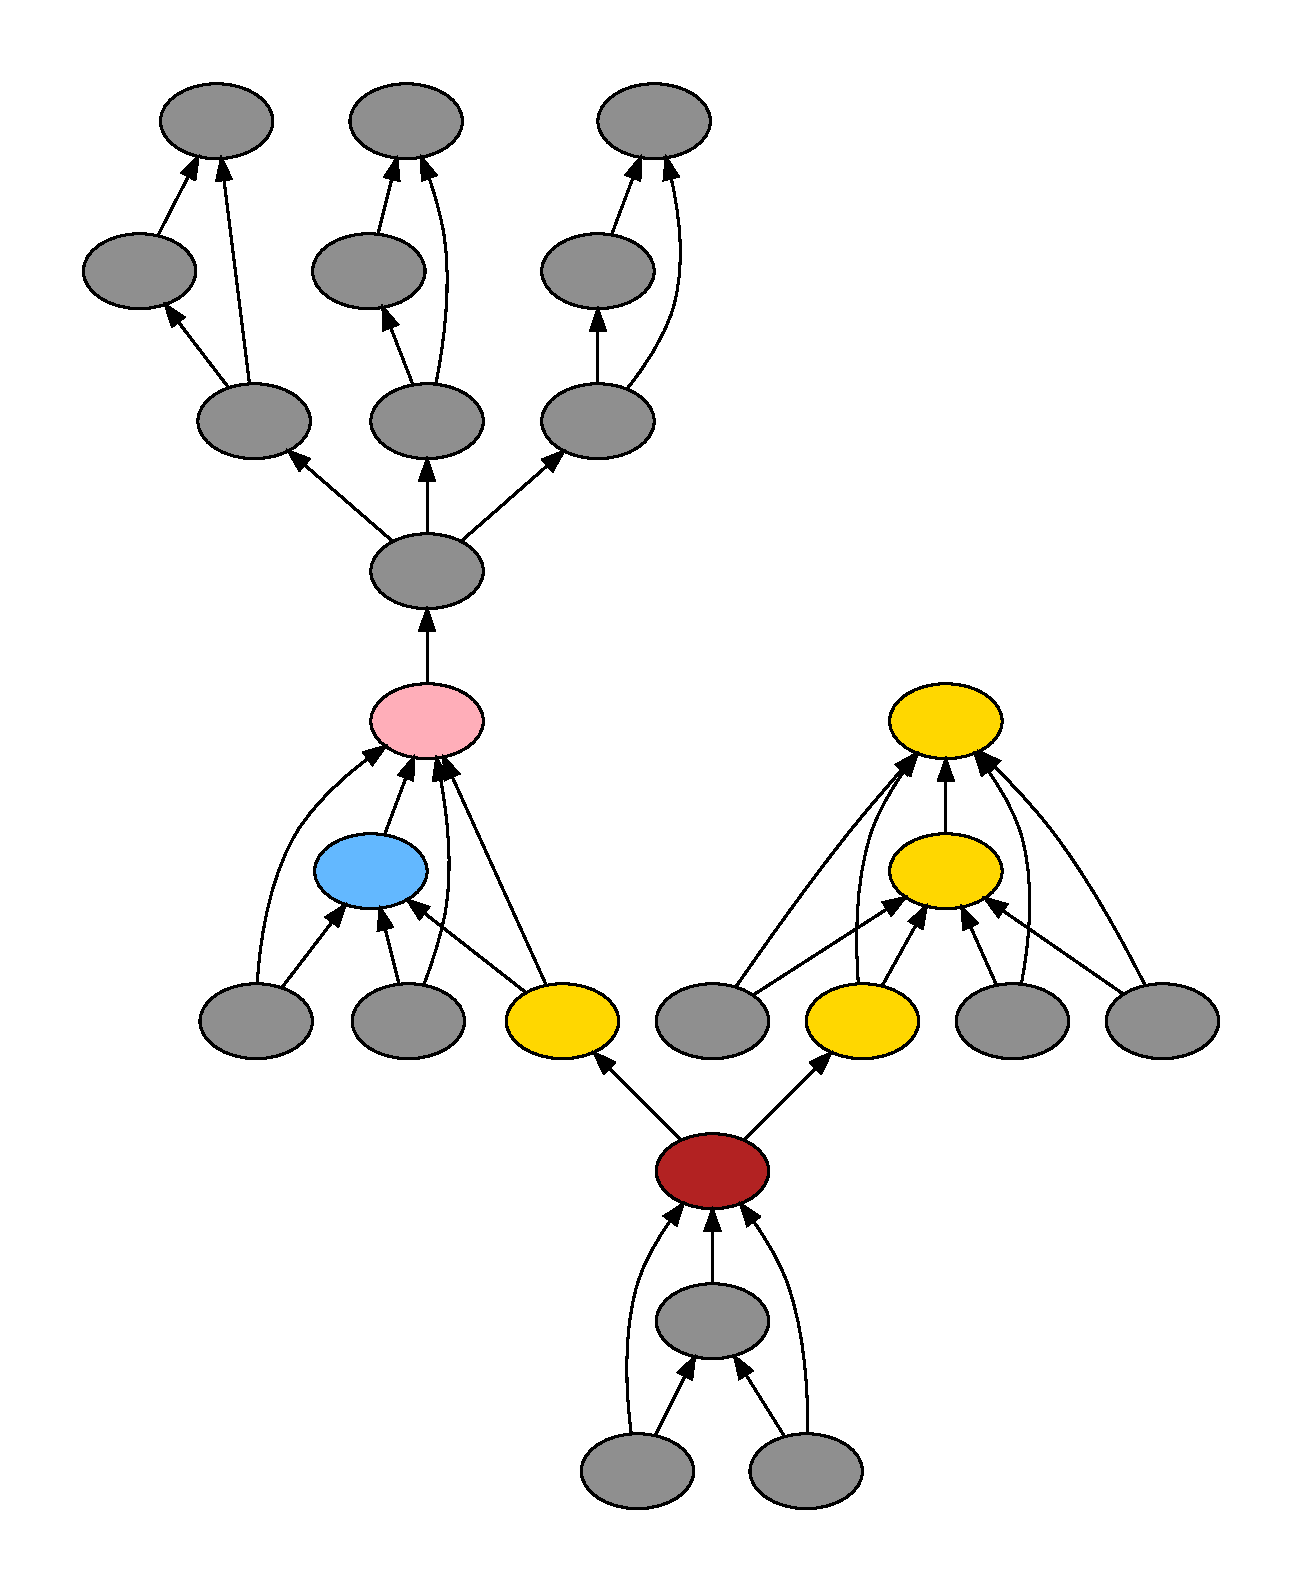
\includegraphics[width=200pt,height=200pt]{aaa_challenge_with_aaa/dot6.pdf}
\label{fig:aaa_challenge_torus}

}

\quad

\subfigure
[
A simulation request may lookup that child before the aaa node has been regenerated, and call regen on it. Regen is normally a no-op for nodes that are not in the drg, but even though the child is not in the drg, it and its parent must be regenerated nonetheless. Thus we need to add the child to the drg dynamically.
]
{
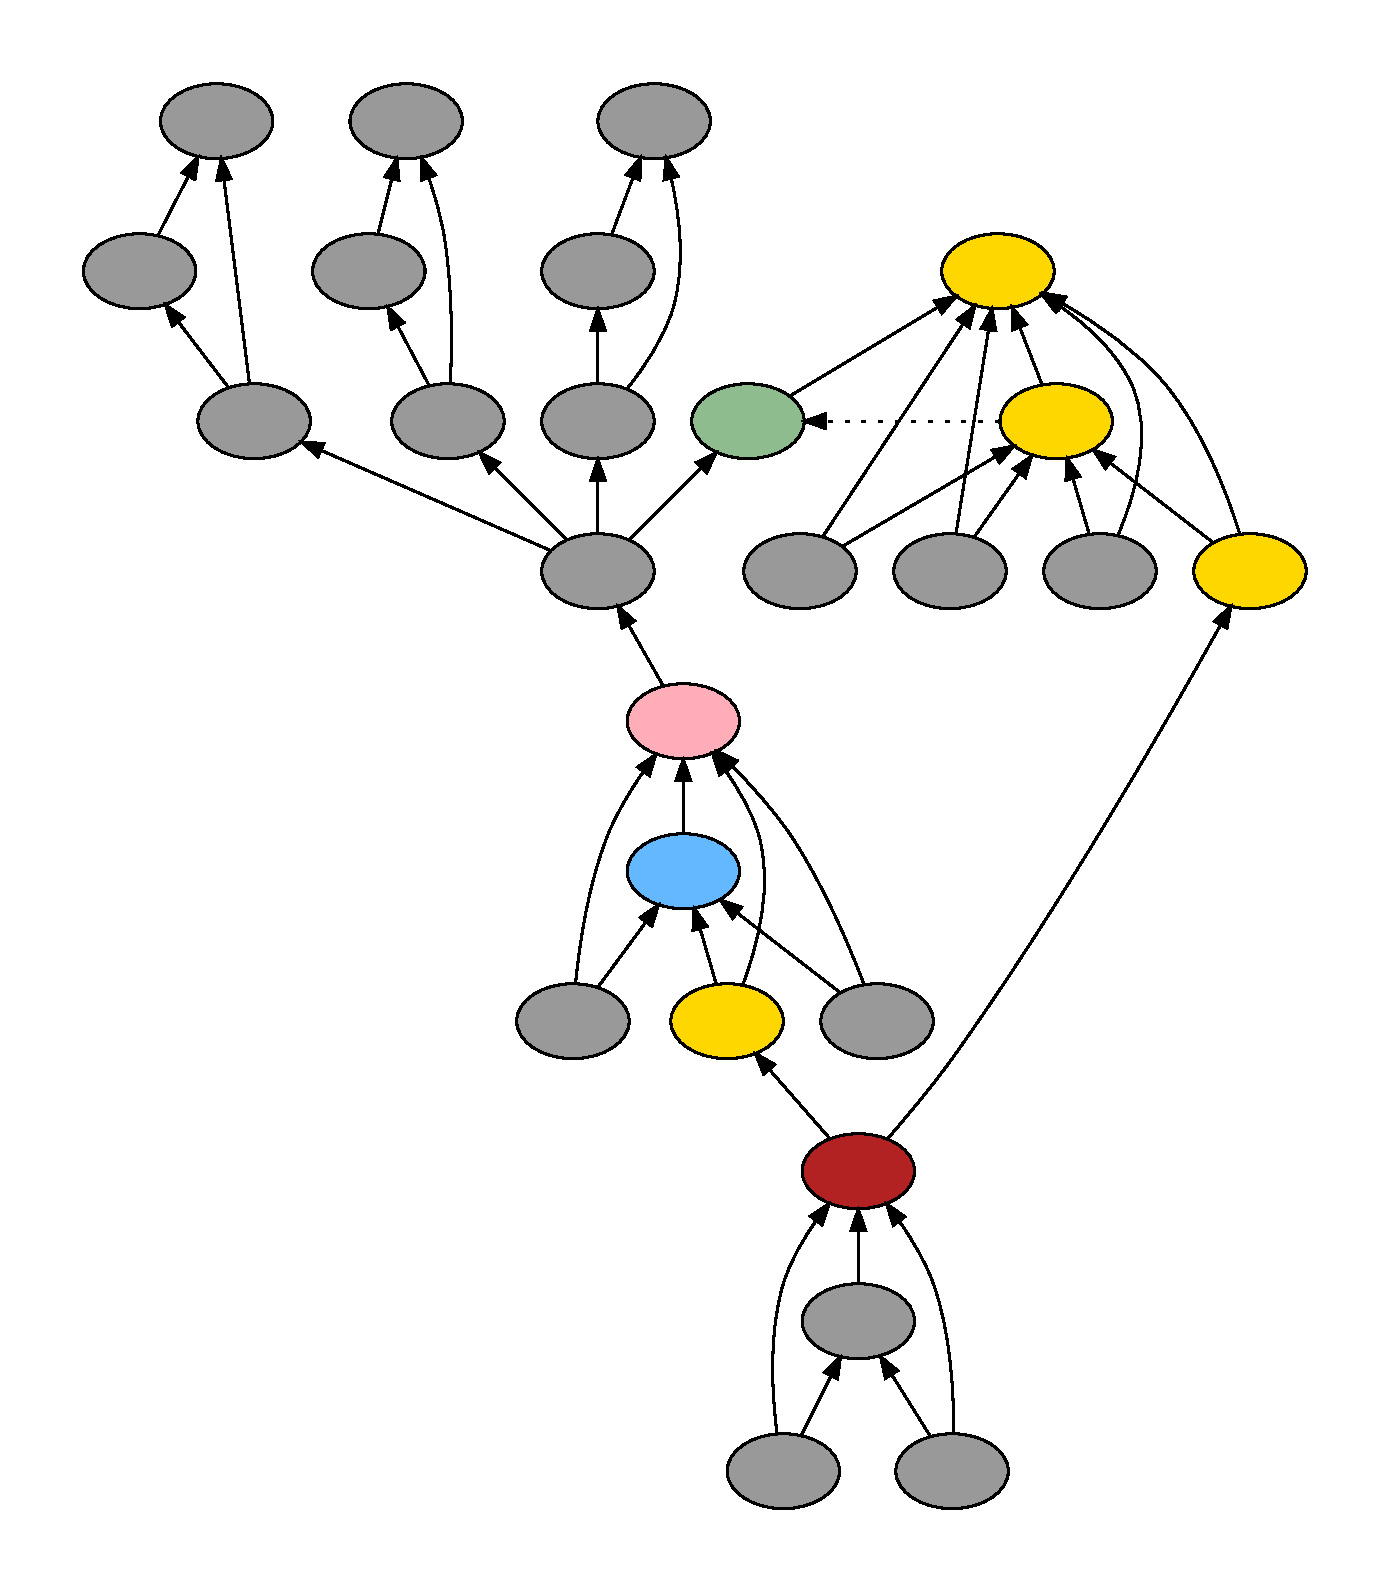
\includegraphics[width=200pt,height=200pt]{aaa_challenge_with_aaa/dot2.pdf}
\label{fig:aaa_challenge_sub}

}
%

\caption{Challenges with absorbing at applications}

\label{fig:aaa_challenge}
\end{figure}


\end{document}
